\documentclass{ctexart}
\usepackage{EC}
\begin{document}
\section{硫及其化合物}
\subsection{单质硫}
\subsubsection{\ce{S8}:$\alpha$-正交硫,$\beta$-单斜硫和$\gamma$-单斜硫}
\begin{substance}[正交$\mbf{\alpha}$-\ce{S8}]
    硫最常见的,也是热力学上最稳定的单质为正交$\mbf{\alpha}$-\ce{S8}(简称正交硫).这是一种黄色固体,具有优良的绝缘性和绝热性.
\end{substance}
正交硫中含有$D_{4\text d}$点群的\ce{S8}分子,其结构颇像皇冠.
\begin{figure}[H]
    \centering
    \subfigure[\ce{S8}分子的俯视图]{
        \begin{minipage}[b]{.45\linewidth}
            \centering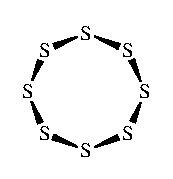
\includegraphics{picture/S8-1.eps}
        \end{minipage}
    }
    \subfigure[\ce{S8}分子的侧视图]{
        \begin{minipage}[b]{.45\linewidth}
            \centering
\includegraphics{picture/S8-2.eps}
        \end{minipage}
    }
    \caption{\ce{S8}分子的立体结构}
\end{figure}
加热$\alpha$-\ce{S8}至$95.3\tccentigrade$可使其转变为$\beta$-单斜\ce{S8}.将硫熔融后缓慢冷却可以得到$\gamma$-单斜\ce{S8}.这两种晶型中都由\ce{S8}分子组成,区别只在于排列方式不同.
\subsubsection{\ce{S6}:$\ep$-硫}
$\ep$-硫由\ce{S6}分子构成,其颜色为橙红色,分子构象与环己烷的椅式六元环一致.这种同素异形体可以由下面的反应制得:
\begin{center}
    \ce{H2S4 + S2Cl2 ->T[\ce{Et2O}] S6 + 2HCl}
\end{center}
\subsection{\ce{S}的小分子:\ce{S2}与\ce{S3}}
低压高温的硫蒸汽中存在\ce{S2}与\ce{S3}分子.\ce{S3}分子呈现樱桃红色,结构与\ce{O3}类似.\ce{S2}分子呈现紫色,结构与\ce{O2}类似.
\subsection{硫的化合物}
\subsubsection{$\mbf{-2}$氧化态}
\paragraph{\ce{H2S}}
我们照例从氢化物开始.
\begin{substance}[\ce{H2S}]
    硫化氢,化学式为\ce{H2S},是无色的具有恶臭的剧毒气体.\ce{H2S}在空气中燃烧时发出浅蓝色的火焰.\ce{H2S}易溶于水,室温下在纯水中的溶解度大约为$1\text{ mol}\cdot\text{L}^{-1}$.
\end{substance}
\ce{H2S}是较弱的酸,并且是一种中等强度的还原剂.将\ce{H2S}溶液置于空气中,溶液将缓慢地变浑浊,其中生成了\ce{S}单质沉淀.
\subsubsection{$\mbf{+4}$氧化态}
\subsubsection{$\mbf{+6}$氧化态}
\subsubsection{多硫阴离子}
\subsubsection{硫代硫酸及其盐}
\subsubsection{连硫酸及其盐}
\subsubsection{连二亚硫酸及其盐}
\subsubsection{$\mbf{+1}$氧化态}
\subsubsection{硫的卤化物与卤氧化物}
\paragraph{硫的氟化物} 硫的氟化物的性质和其它卤素的卤化物有一定程度的区别,因此分开讨论.
\begin{enumerate}[label=\tbf{\arabic*},topsep=0pt,parsep=0pt,itemsep=0pt,partopsep=0pt]
    \item \tbf{\ce{S2F2}}\\
        硫和\ce{AgF}在干燥的容器中氟化可以得到\ce{FSSF}.在有碱金属氟化物存在时,这种物质容易异构化形成\ce{SSF2}.这是一个简单的键合异构的例子.当然,\ce{SSF2}本身也可以由\ce{SO2}溶剂中的\ce{KF}与\ce{S2Cl2}反应得到:
        \begin{center}
            \ce{2KSO2F + S2Cl2 ->T[\ce{SO2}] SSF2 + 2KCl + 2SO2}
        \end{center}
        两者的结构示意如下.
        \begin{figure}[H]
            \centering
            \subfigure[\ce{FSSF}的结构]{
                \begin{minipage}[b]{.45\linewidth}
                    \centering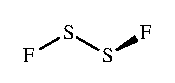
\includegraphics{picture/S2F2.eps}
                \end{minipage}
            }\subfigure[\ce{SSF2}的结构]{
                \begin{minipage}[b]{.45\linewidth}
                    \centering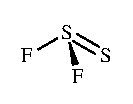
\includegraphics{picture/SSF2.eps}
                \end{minipage}
            }
            \caption{两种\ce{S2F2}的结构}
        \end{figure}
    \item \tbf{\ce{SF2}}\\
        \indent \ce{SF2}的稳定性并不如与它相似的\ce{H2S}或\ce{SCl2},因而难以得到.这种化合物需要\ce{KF}对\ce{SCl2}氟化后的一系列硫的氟化物中分离制得.
    \item \tbf{\ce{SF4}}\\
        \indent 相比前面几种物质,\ce{SF4}是一种稳定得多的氟化物.\ce{SF4}最好由下面的方法制备:
        \begin{center}
            \ce{3SCl2 + 4NaF ->T[\ce{MeCN}][$75\tccentigrade$] S2Cl2 + SF4 + 4NaCl}
        \end{center}
        它具有经典的跷跷板结构,其中的四个\ce{F}是不断流变的.有关\ce{SF4}的有趣的衍生结构是\ce{(H2C)SF4},它和\ce{SOF4}一样具有三角双锥结构,轴向的\ce{F}向远离端基\ce{O}或\ce{CH2}的方向偏移.值得注意的是,\ce{CH2}中的两个\ce{H}与轴向\ce{F}共平面,这是由于$\pi$键对轨道方向的要求决定的,尽管此时看起来位阻更大.
        \begin{figure}[H]
            \centering
            \subfigure[\ce{SF4}的结构]{
                \begin{minipage}[b]{.3\linewidth}
                    \centering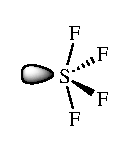
\includegraphics{picture/SF4.eps}
                \end{minipage}
            }
            \subfigure[\ce{SOF4}的结构]{
                \begin{minipage}[b]{.3\linewidth}
                    \centering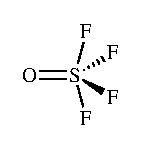
\includegraphics{picture/SOF4.eps}
                \end{minipage}
            }
            \subfigure[\ce{(H2C)SF4}的结构]{
                \begin{minipage}[b]{.3\linewidth}
                    \centering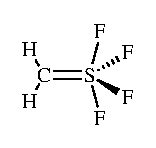
\includegraphics{picture/S(CH2)F4.eps}
                \end{minipage}
            }
            \caption{\ce{SF4}及其衍生物的结构}
        \end{figure}
        \ce{SF4}遇潮气迅速分解,并立即水解生成\ce{HF}和\ce{SO2}.尽管如此,在无机和有机合成中,它仍是具有高度选择性的强氟化剂,用途颇为广泛.
    \item \tbf{\ce{SF6}}\\
        \indent 六氟化硫\ce{SF6}可由硫在氟气氛中燃烧制得.它是无色,无臭,无味,无毒的气体\footnote{少量吸入\ce{SF6}可以让声音变得粗犷,这和吸入\ce{He}使得声音变细正好相反.请勿自行尝试此实验,以避免窒息风险.},无反应性和可燃性,也无溶解性.正由于它突出的稳定性和优良的绝缘性,广泛用作高压发电机和开关装置中的绝缘气体.\\
        \indent 近年来的最新观点认为\ce{SF6}中的\ce{S}并非VSEPR理论所认为的$\text{d}^2\text{sp}^3$杂化,而是采取sp杂化与两个\ce{F}成键,其余四个\ce{F}则与\ce{S}通过电性作用结合.经过平均化后,形成了正八面体的\ce{SF6}分子.
    \item \tbf{\ce{S2F10}}\\
        \indent 对硫的不完全氟化可以得到\ce{S2F10}分子.它的结构可以看作是两个\ce{SF6}各自去掉一个\ce{F}后两个\ce{S}相连的结果.由于没有特别的轨道作用,为了避免位阻,\ce{S2F10}采取交错式结构,其中的\ce{S-S}键也较长且弱.\\
        \indent \ce{S2F10}的反应性介于\ce{SF4}与\ce{SF6}之间.。它不为水所水解,甚至不为稀酸或稀碱所水解,这一点和\ce{SF4}不同;它作为剧毒物质也不同于\ce{SF6}.\ce{S2F10}在$15\tccentigrade$时迅速发生歧化,分解生成\ce{SF4}和\ce{SF6}.\\
        \indent \ce{S2F10}可以在丙酮溶液中氧化\ce{KI}而析出\ce{I2}.一个小把戏是还原产生的\ce{SF4}可以对丙酮进行氟化,因此反应的方程式应当为:
        \begin{center}
            \ce{S2F10 + 2KI + 4Me2CO -> 2SO2 + 2KF + I2 + 4Me2CF2}
        \end{center}
        下面是\ce{SF6}和\ce{S2F10}的结构.
        \begin{figure}[H]
            \centering
            \subfigure[\ce{SF6}的结构]{
                \begin{minipage}[b]{.45\linewidth}
                    \centering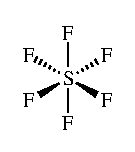
\includegraphics{picture/SF6.eps}
                \end{minipage}
            }
            \subfigure[\ce{S2F10}的结构]{
                \begin{minipage}[b]{.3\linewidth}
                    \centering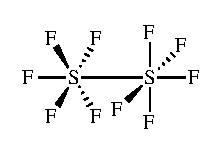
\includegraphics{picture/S2F10.eps}
                \end{minipage}
            }
            \caption{\ce{SF6}和\ce{S2F10}的结构}
        \end{figure}
\end{enumerate}
\paragraph{硫的氯化物}
在剩余的硫的卤化物中,我们主要讨论最常见的\ce{SCl2}和\ce{S2Cl2},它们都是重要的化工产品.
\begin{substance}[\ce{SCl2}]
    二氯化硫,化学式为\ce{SCl2},是有毒且有恶臭味的樱桃红色液体,易挥发,熔点为$-122\tccentigrade$,沸点为$59\tccentigrade$.
\end{substance}
\begin{substance}[\ce{S2Cl2}]
    二氯化二硫,化学式为\ce{S2Cl2},是有毒且有恶臭味的金黄色液体,熔点为$-76\tccentigrade$,沸点为$138\tccentigrade$.
\end{substance}
\subsubsection{硫的氮化物}
\subsubsection{硫的多原子阳离子}
为了保持连续性,这部分内容将和\ce{Se},\ce{Te}的多原子阳离子一起介绍.
\end{document}